\chapter{Wstępne planowanie}

\section{Analiza dostępnych aplikacji}

Poniżej przedstawiono 2 najbardziej popularne serwisy internetowe oferujące materiały oraz narzędzia do gry na gitarze. 

\subsection{Guitar Tuna}

Jedną z większych i najbardziej spopularyzowanych aplikacji jest Guitar Tuna, przeznaczona ona jest w głównej mierze na urządzenia mobilne, z ograniczoną ilością funkcjonalności na urządzenia desktopowe. Do dostępnych narzędzi zalicza się:

\subsubsection{Stroik}

Stroik gitarowy, z graficzną reprezentacją tonu oraz "odległości" od domniemanej nuty. Narzędzie umożliwia parametryzację polegającą na wyborze docelowej nuty do jakiej chcemy dostroić instrument. Narzędzie umożliwia też wybór instrumentu, wraz z jego graficzną reprezentacją na ekranie i przypisanymi nazwami nut obok odpowiadających pokręteł. Użytkownik do wyboru ma takie instrumenty jak gitara, ukulele, gitara basowa. Dodatkowym atutem jest możliwość wyboru niestandardowych strojeń instrumentów. 

% \begin{figure}[htb]
% 	\centering
% 	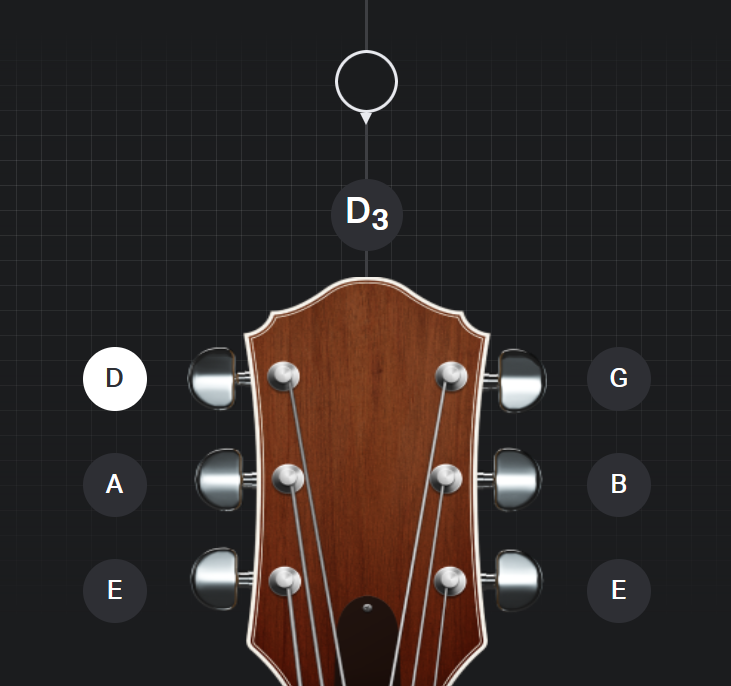
\includegraphics[width=.7\linewidth]{rysunki/GTSTROIK}
% 	\caption{Stroik aplikacji Guitar Tuna} \label{fig:pageLayout}
% \end{figure}

\subsubsection{Akordy}

Sekcja akordów witryny internetowej jest uboższa aniżeli w aplikacji mobilnej. Narzędzie to daje dostęp do licznych piosenek, przy których przedstawione zostały akordy potrzebne do ich zagrania, wraz z tekstem i przejściami akordów w odpowiednich momentach. Zostało to zrobione statycznie, bez informacji na temat tempa utworu, czy dynamiki przejść pomiędzy granymi akordami. Istnieje tu również myląca funkcja "smart scroll" sugerująca możliwość grania wraz z podkładem grającym w tle, po naciśnięciu przycisku pojawia się jedynie odnośnik do pobrania aplikacji mobilnej.

% \begin{figure}[htb]
% 	\centering
% 	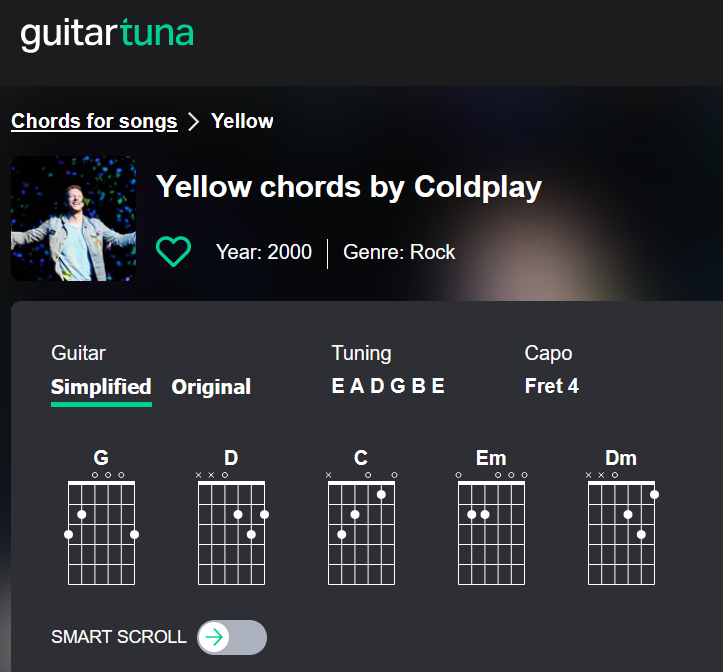
\includegraphics[width=.7\linewidth]{rysunki/ChordsGT}
% 	\caption{Sekcja akordów aplikacji Guitar Tuna} \label{fig:pageLayout}
% \end{figure}

\subsubsection{Podsumowanie aplikacji Guitar Tuna}

Aplikacja sama w sobie jest bardzo przystępna i intuicyjna, największym atutem jest stroik dajacy dowolność jeżeli chodzi o używany instrument. Wersja desktopowa jest jednak znacznie okrojona w porównaniu do aplikacji mobilnej, nie znajdziemy tu listy akordów, diagramów skal czy metronomu. 

\subsection{Truefire}

Aplikacja ta zawiera w większości płatne lekcje i materiały edukacyjne do gry na gitarze takie jak:

\begin{itemize}
    \item podkłady muzyczne do gry,
    \item kursy nauki gry poszczególnych stylów muzycznych np. blues, funk czy jazz,
    \item możliwość wykupienia prywatnych lekcji u instruktorów,
    \item transkrypcje znanych piosenek z instrukcjami gry,
\end{itemize}

Poza tym sama witryna zawiera sekcję z narzędziami do nauki, na podstawie której przeprowadzono analizę pod względem użyteczności, łatwości przekazu, sposobu przedstawienia poszczególnych elementów. 

\subsubsection{Stroik}

Pierwszym narzędziem jest stroik gitarowy, który został skonstruowany w sposób prosty, rozpoznaje poszczególne dźwięki skali chromatycznej. Zawiera on w sobie "input meter", będący indykatorem poziomu decybeli dostarczanych do mikrofonu. Ma on również slider umożliwiający parametryzację czułości mikrofonu. Samo narzędzie naturalnie umożliwia dostrojenie gitary do poszczególnych dźwięków, może być ono natomiast mało intuicyjne dla początkujących graczy, którzy nie są zapoznani z domyślnym strojeniem strun gitary.
% \begin{figure}[htb]
% 	\centering
% 	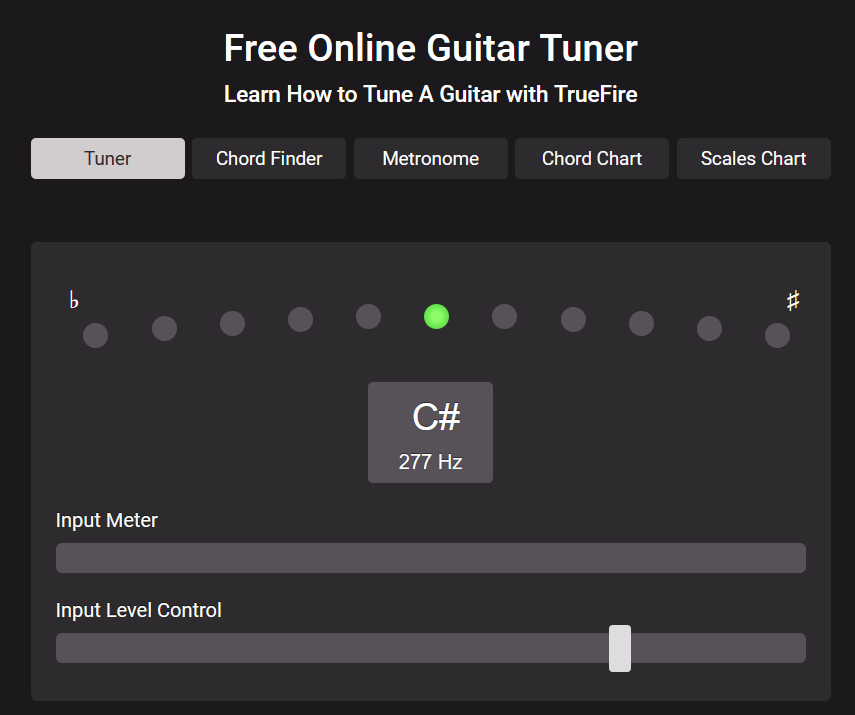
\includegraphics[width=.7\linewidth]{rysunki/tuneFireStroik}
% 	\caption{Stroik aplikacji Truefire} \label{fig:pageLayout}
% \end{figure}

\subsubsection{Eksplorator akordów}

Drugim z pięciu dostępnych narzędzi jest eksplorator akordów, który na podstawie zaznaczonych pozycji naciśniętych progów przeszukuje dostępne możliwe akordy, wyświetlając przy tym te będące najbardziej podobne do zaznaczonych pozycji. Samo narzędzie jest z całą pewnością bardzo kreatywne. Jeżeli chodzi o samą naukę narzędzie wydaje się być mało przydatne, z racji braku kontekstu przy wyświetlanych znalezionych akordach, nie podając informacji odnośnie skal, do których sam akord należy. Ze względu na algorytm dopasowujący nawet w przypadku, gdy podamy losową pozycję naciśniętych progów, wyświetlone i tak zostana prawidłowe akordy. Narzędzie może być mylące dla nowych graczy, mogących założyć, że podany przez nich układ wpisuje się pod prawidłowe akordy uznawane przez teorię muzyki.
% \begin{figure}[htb]
% 	\centering
% 	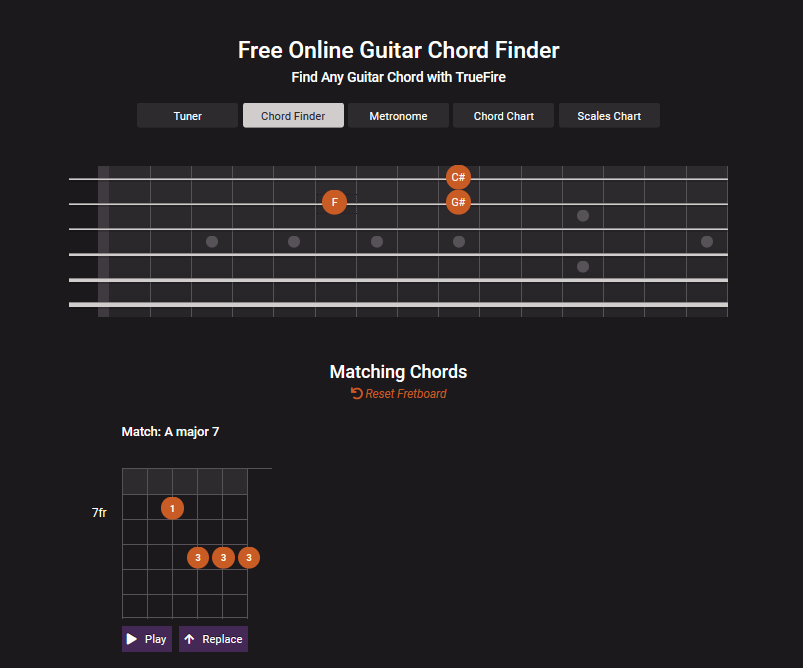
\includegraphics[width=.7\linewidth]{rysunki/ChordFinder}
% 	\caption{Eksplorator akordów aplikacji TrueFire} \label{fig:pageLayout}
% \end{figure}

\subsubsection{Metronom}

Metronom zaimplementowany jest w sposób prosty, dostarczając wszystkie potrzebne funkcjonalności w jasny i przejrzysty sposób. Dla użytkownika dostępne są funkcje zmiany tempa wybijania poszczególnych beatów, możliwość ręcznego ustawienia tempa, oraz dobór metrum z listy 6 dostępnych. Sama realizacja tej funkcjonalności, mogłaby zawierać dodatkowo opcję wyboru całych nut, a nie jedynie pół nut i ósemek przy wyborze metrum, poza tym samo narzędzie wykonuje swoje zadanie, umożliwiając treningu rytmu.
% \begin{figure}[htb]
% 	\centering
% 	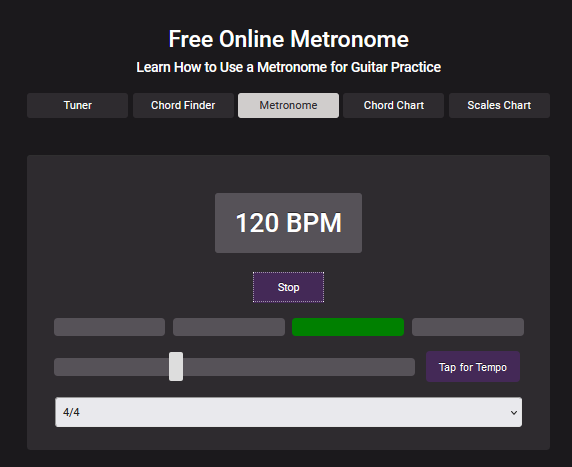
\includegraphics[width=.7\linewidth]{rysunki/METRO}
% 	\caption{Metronom aplikacji TrueFire} \label{fig:pageLayout}
% \end{figure}

\subsubsection{Księga akordów}

Funkcjonalność księgi akordów zaprezentowana została w mało przystępny sposób, mianowicie prezentowany nam jest diagram w postacie statycznego obrazka, z mało czytelnym podziałem pomiędzy poszczególnymi akordami. Diagram ten jest wadliwy z powodu jego nieczytelności, może on być niezrozumiały dla graczy początkujących jak i średnio zaawansowanych, z powodu braku kontekstu pod akordami. Same diagramy nie obrazują numeru progu, na którym dany akord ma być grany oraz nie przedstawia nuty odpowiadającej danej strunie.
% \begin{figure}[htb]
% 	\centering
% 	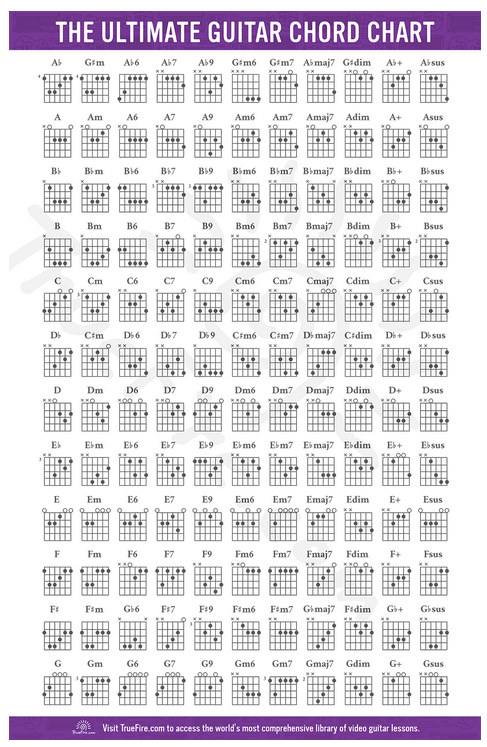
\includegraphics[width=.7\linewidth]{rysunki/ChordChart}
% 	\caption{Lista akordów aplikacji Tunefire} \label{fig:pageLayout}
% \end{figure}

\subsubsection{Diagramy skal}

Ostatnim narzędziem dostępnym dla użytkownika są diagramy skal, przedstawiane jest 6 najpopularniejszych skal muzycznych, brakuje jednak możliwości przeniesienia tych diagramów poprzez gryf, wraz z informacją na temat tego w jakiej skali grany miałby być poszczególny diagram. Jest to rozwiązanie wadliwe, nie dostarczające wystarczająco dużej ilości informacji. 

% \begin{figure}[htb]
% 	\centering
% 	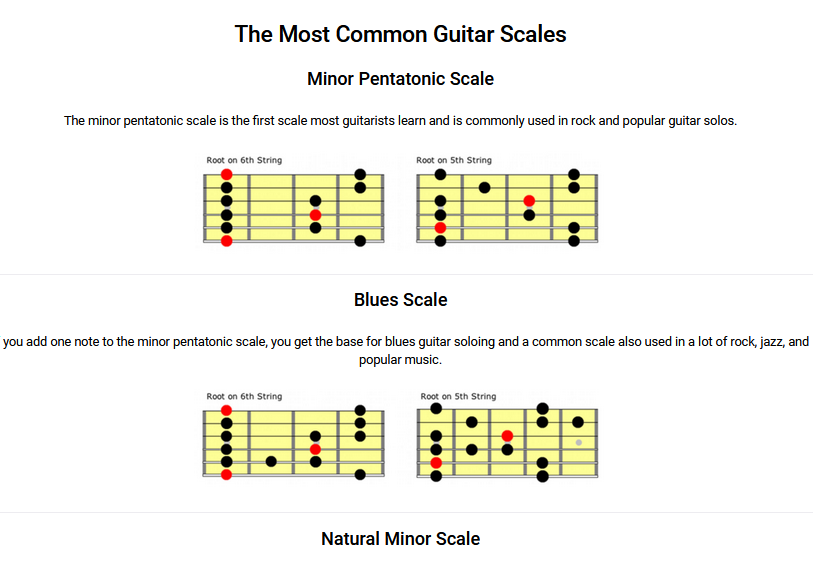
\includegraphics[width=.7\linewidth]{rysunki/SKALETF}
% 	\caption{Kontrola marginesów i odstępów elementów na stronie} \label{fig:pageLayout}
% \end{figure}

\subsubsection{Podsumownanie narzędzia Truefire}

Narzędzie w ogólnym ujęciu jest dobre, dostarcza podstawowe funkcjonalności umożliwiające naukę gry na gitarze, trening rytmu oraz możliwość dostrojenia samego instrumentu. Same funkcjonalności natomiast zostawiają dużo miejsca na rozwój, możliwość parametryzacji czy też umieszczenie informacji kontekstowych, oraz objaśnienie pewnych sformułowań związanych z pozycjami akordów na gryfie. Narzędzie wyszukiwania akordów na podstawie podanych numerów progrów jest natomiast samo w sobie bardzo mylące. Najbardziej przydatnym narzędziem z całego zestawienia jest metronom, będący prosty w obsłudze i dający możliwość prostego treningu rytmu grania. 

\section{Podsumowanie analizy aplikacji}

Biorąc pod uwagę powyżej wymienione aplikacje, wyciągnięto wnioski odnośnie ich najlepszych cech oraz niedoskonałości. Do dobrych cech aplikacji można zaliczyć prostotę ich obsługi, zwłaszcza w funkcjonalności stroika aplikacji Guitar Tuna oraz metronomu Tunefire. Do największych wad należy brak kontekstu przy wizualizacji listy dostępnych akordów, oraz ograniczoną ilość możliwości przy wersji desktopowej aplikacji. Na tej podstawie wyciągnięto aspekty, oraz narzędzia jakie znajdą się w docelowym produkcie, mianowicie:

\begin{itemize}
	\item prosty w obsłudze metronom z możliwością doboru tempa oraz metrum gry,
	\item stroik umożliwiający wybór nuty, do której docelowo strojony jest instrument,
	\item księgę akordów z podpisanym akordem, w to wchodzi wariancja akordu oraz ton w jakiej jest on grany,
	\item koło kwintowe reprezentujące w przejrzysty sposób skale muzyczne.
\end{itemize}

\section{Makieta aplikacji}

Makieta aplikacji utworzona została za pomocą oprogramowania figma, przedstawia ona podstawowy koncept, oraz zarys sekcji aplikacji. Na poszczególnych obrazkach można zobaczyć wizualizacje scen, zaczynając od głównego ekranu, stroika, metronomu, koła kwintowego, księgi akordów, kończąc na treningu słuchu. 

%\begin{figure}[htb]
	%\centering
	%\includegraphics[width=.7\linewidth]{rys03/pageLayout2}
	%\caption{Kontrola marginesów i odstępów elementów na stronie} \label{fig:pageLayout}
%\end{figure}

%\begin{figure}[htb]
	%\centering
	%\includegraphics[width=.7\linewidth]{rys03/pageLayout2}
	%\caption{Kontrola marginesów i odstępów elementów na stronie} \label{fig:pageLayout}
%\end{figure}

%\begin{figure}[htb]
	%\centering
	%\includegraphics[width=.7\linewidth]{rys03/pageLayout2}
	%\caption{Kontrola marginesów i odstępów elementów na stronie} \label{fig:pageLayout}
%\end{figure}

%\begin{figure}[htb]
	%\centering
	%\includegraphics[width=.7\linewidth]{rys03/pageLayout2}
	%\caption{Kontrola marginesów i odstępów elementów na stronie} \label{fig:pageLayout}
%\end{figure}

%\begin{figure}[htb]
	%\centering
	%\includegraphics[width=.7\linewidth]{rys03/pageLayout2}
	%\caption{Kontrola marginesów i odstępów elementów na stronie} \label{fig:pageLayout}
%\end{figure}

\section{Projekt graficznego interfejsu użytkownika}

Projekt gui użytkownika utworzony w aplikacji figma obejmuje utworzenie:

\begin{itemize}
	\item grafik przycisków dla poszczególnych scen,
	\item graficznych tytułow poszczególnych scen,
	\item elementów wizualizujących poszczególne funkcjonalności np: akordy gitarowe, takty metronomu,
	\item tło oraz elementy kontekstowe ułatwiające posługiwanie się aplikacją.
\end{itemize}

Poszczególne zaprojektowane elementy prezentują się następująco, na poniższych grafikach przedstawiono: projekt przycisków, tytułów scen oraz przykładów reprezentacji akordów na gryfie. 

%\begin{figure}[htb]
	%\centering
	%\includegraphics[width=.7\linewidth]{rys03/pageLayout2}
	%\caption{Kontrola marginesów i odstępów elementów na stronie} \label{fig:pageLayout}
%\end{figure}

%\begin{figure}[htb]
	%\centering
	%\includegraphics[width=.7\linewidth]{rys03/pageLayout2}
	%\caption{Kontrola marginesów i odstępów elementów na stronie} \label{fig:pageLayout}
%\end{figure}

%\begin{figure}[htb]
	%\centering
	%\includegraphics[width=.7\linewidth]{rys03/pageLayout2}
	%\caption{Kontrola marginesów i odstępów elementów na stronie} \label{fig:pageLayout}
%\end{figure}

\section{Projekt architektury aplikacji}

Projekt architektury dla aplikacji stworzony został w sposób taki, aby każda z poszczególnych funkcjonalności była przejrzysta, a sama aplikacja umożliwiała płynne przełączanie pomiędzy sekcjami aplikacji. Zastosowano wzorzec Model-View-ViewModel, umożliwiający rozdzielenie logiki aplikacji, interfejsu oraz zarządzania danymi. 

%\begin{figure}[htb]
	%\centering
	%\includegraphics[width=.7\linewidth]{rys03/pageLayout2}
	%\caption{Kontrola marginesów i odstępów elementów na stronie} \label{fig:pageLayout}
%\end{figure}

W skład wzorca wchodzą poniższe 3 elementy:
\begin{itemize}
	\item Model: Logika danych aplikacji, zawierająca dane akordów, dźwięków, tempo metronomu,
	\item View: Zawierająca sceny samej aplikacji, dla każdej z funkcjonalności zaplanowany jest osobny widok (sceny),
	\item ViewModel: Do każdej ze scen przypisany został kontroler odpowiedniej sceny umożliwiający komunikację pomiędzy widokiem, a modelem, zawiera on logikę aplikacji oraz funkcji potrzebnych w danej scenie.
\end{itemize}

\subsection{Projekt poszczególnych scen}

W tej sekcji przedstawiono projekt dla każdej z funkcjonalności aplikacji, rozrysowując przy tym komponenty wchodzące w skład danego narzędzia, wraz z ich celem, sposobem implementacji, technologiami użytymi do stworzenia poszczególnych elementów. 

\subsubsection{Scena 1: Scena Główna}

\begin{itemize}

\item Cel: Reprezentacja możliwości wyboru, oraz udzielenie użytkownikowi dostępu do poszczególnych narzędzi za pomocą czytelnych przycisków, które po naciśnięciu przechodzą do odpowiadającej im sceny z danym narzędziem. 
\item Komponenty: Elementami wchodzącymi w skład sceny głównej, jest 5 przycisków: stroik, metronom, koło kwintowe, księga akordów, trening słuchu. Dodatkowo scena główna zawiera obiekt tekstowy z logiem aplikacji.  
\item Technologie: Do realizacji tej oto sceny użyto wbudowaną bibliotekę w silnik Unity, a mianowicie Unity.UI, umożliwiającą utworzenie graficznego interfejsu uzytkownika. 
\item Komunikacja: Każdy z przycisków wchodzących w skład sceny podłączony jest pod kontroler sceny, służący jako pośrednik, w skrypcie należącym do kontrolera poszczególnym przyciskom przypisywana jest funkcja odpowiadająca za załadowanie odpowiedniej sceny. 
\end{itemize}

\subsubsection{Scena 2: Stroik}

\begin{itemize}
\item Cel: Udostępnienie możliwości nastrojenia gitary poprzez wybór docelowej struny, do której użytkownik chce nastroić instrument. Następnie zagrane przez użytkownika dźwięki analizowane będą, a wyniki analizy reprezentowane zostaną jako informacja odnośnie tego, czy ton należy obniżyć czy podwyższyć.
\item Komponenty: W skład sceny wchodzi mikrofon, analizator dźwięku, przyciski odpowiadające strunom na gitarze, oraz wizualizator aktualnego poziomu nastrojenia instrumentu.  
\item Technologie: Do użytych technologii wykorzystano bibliotekę opartą na otwartej licencji służącą do analizy dostarczanego dźwięku, oraz wyciągnięcie z niego częstotliwości zagranej nuty. Dodatkowo do stworzenia graficznego interfejsu posłużono się biblioteką Unity.UI.   
\item Komunikacja: Użyto kontroler sceny, aby umożliwić komunikacje pomiędzy elementami graficznymi a analizatorem dźwięku. 
\end{itemize}

\subsubsection{Metronom}

\begin{itemize}
\item Cel: Zapewnienie użytkownikowi możliwości treningu rytmu podczas gry, poprzez reprezentację poszczególnych taktów zsynchronizowanych z dźwiękiem "bitu".
\item Komponenty: Do realizacji tej sceny zastosowano przyciski umożliwiające parametryzację taktu, oraz bpm(ang. beats per minute). Wizualizacja metronomu odbywa się za pośrednictwem pojawiających się na ekranie kwadratów reprezentujących poszczególny takt, które zmieniają swoje kolory z białego na czarny, wraz z czasem wybijania danego rytmu.
\item Technologie: Skrypt napisany w języku C\# realizujący logikę działania metronomu.
\item Komunikacja: Poszczególne komponenty komunikują się ze sobą za pośrednictwem kontrolera sceny metronomu, zawierający odwołania do poszczególnych komponentów.
\end{itemize}

\subsubsection{Księga akordów}

\begin{itemize}
\item Cel: Wizualizacja pozycji akordów na gryfie, dla każdej nut, wraz z możliwymi wariancjami akordów.
\item Komponenty: Do komponentów należą przyciski odpowiadające za przeglądanie listy dostępnych akordów, element graficzny wizualizujący aktualnie wybrany akord, wraz z przyciskami odpowiadającymi za przełączenie sceny do widoku diagramu wszystkich możliwych akordów.
\item Technologie: Wbudowana biblioteka do obsługi graficznego interfejsu użytkownika - Unity.UI.
\item Komunikacja: Komponenty komunikują się ze sobą za pomocą menadżera sceny, przechowującego za pomoca listy graficzne reprezentacje akordów, które wyświetlane są w odpowiednich momentach. 
\end{itemize}

\subsubsection{Trening słuchu}

\begin{itemize}
\item Cel: Umożliwienie użytkownikowi przeprowadzenie ćwiczeń mających na celu nabycia umiejętności rozpoznawania granej nuty za pomocą samego słuchu.
\item Komponenty: Przycisk odpowiadający za odegranie losowo jednej z 12 nut skali chromatycznej, przyciski odpowiadające za odpowiedź, po naciśnięciu których weryfikowana jest poprawność udzielonej odpowiedzi. Scena zawiera również system audio odpowiadający za odegranie dźwięku
\item Technologie: Za odgrywanie dźwięków odpowiada biblioteka Unity.Sound, wraz z gotowym komponentem audio wbudowanym w silnik Unity.
\item Komunikacja: Za komunikację pomiędzy komponentami odpowiada menadzer sceny, łączący ze sobą przyciski, zawierający logike odpowiedzialną za działanie sceny.
\end{itemize}

\subsubsection{Koło kwintowe}

\begin{itemize}
	\item Cel: Wizualizacja koła kwintowego, wraz z skalą molową i durową.
	\item Komponenty: Elementy graficzne, w postaci przycisków, zawierające komponent image, który zawiera odpowiadającą nutę.
	\item Technologie: Użyto biblioteki Unity.UI do reprezentacji poszczególnych nut.
	\item Komunikacja: Komunikacja odbywa się poprzez menadżer sceny, zawierający logikę odpowiadającą za podświetlenie odpowiadających nut po naciśnięciu jednego z przycisków na kole kwintowym
\end{itemize}
